\documentclass[10pt]{article}
\usepackage{fontspec}
\usepackage[utf8]{inputenc}
\setmainfont{Didot}
%\usepackage[papersize={11in, 17in}]{geometry}
\usepackage[paperwidth=11in,paperheight=17in,margin=1in,headheight=0.0in,footskip=0.5in,includehead,includefoot,portrait]{geometry}
\usepackage[absolute]{textpos}
\TPGrid[0.5in, 0.25in]{23}{24}
\parindent=0pt
\parskip=12pt
\usepackage{nopageno}
\usepackage{graphicx}
\graphicspath{ {./images/} }
\usepackage{amsmath}
\usepackage{tikz}
\newcommand*\circled[1]{\tikz[baseline=(char.base)]{
            \node[shape=circle,draw,inner sep=1pt] (char) {#1};}}

\begin{document}


\begin{textblock}{23}(0, 1)
\begin{center}
\huge FOREWORD
\end{center}
\end{textblock}

\vspace*{0.25\baselineskip}

\begingroup
\begin{center}
\leftskip2in
$Cthar$ is an Aramaic word, pronounced ``seth-ar'' meaning ``to hide'' which can be used as a euphemism meaning ``to disassemble.''
\rightskip\leftskip
\phantom{text} \hfill (G.R.E.)
\end{center}
\endgroup
  
%\vspace*{0.5\baselineskip}

\begin{center}
\huge PERFORMANCE NOTES
\end{center}

\begin{center}
\pmb{Microtones}:
\end{center}

\begin{center}
\includegraphics[width=0.5\textwidth]{microtones.png}
\end{center}

\begin{center}
Accidentals apply only to the pitch which they immediately precede.
\end{center}

\begingroup
\begin{center}
\leftskip1in
\pmb{Bow Contact Points} \hspace{0.3mm} 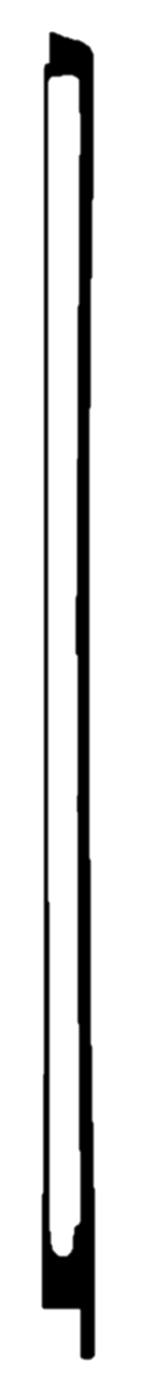
\includegraphics[height=0.020\textheight]{bow_position_tablature.eps} \hspace{0.3mm}: In various passages throughout this piece, there is notation which represents the points along the length of the bow which are touched by the string. These positions are written as fractions where \( \frac{0}{1} \) represents $talon$ and \( \frac{1}{1} \) represents $point$. Passages without these indications should be bowed at the performer's discretion.
\rightskip\leftskip
\phantom{text} \hfill \phantom{()}
\end{center}
\endgroup


\begingroup
\begin{center}
\leftskip1in
\pmb{String Contact Points}: The indications of string contact positions such as $sul \ tasto$ (abbreviated as $st.$), $sul \ ponticello$ (abbreviated as $sp.$), $molto \ sul \ ponticello$ (abbreviated as $msp.$), etc. should be considered as points along the continuum of the length string. The performer should make an effort to smoothly transition from one position to the next throughout the duration of the passage covered by the arrow-demarcated dashed line. When this arrow is not present, the performer should default to an $ordinario$ position. In passages where the ``String Contact Point'' notation is combined with the ``Bow Contact Point'' notation, both motions should be managed independently, therefore if the `BCP' is held static for any duration of time, the `SCP' should still be in motion.
\rightskip\leftskip
\phantom{text} \hfill \phantom{()}
\end{center}
\endgroup

\begingroup
\begin{center}
\leftskip1in
\pmb{Dynamics}: The dynamics indicated concurrently with `Bow Contact Points' should be considered ``effort dynamics.'' As such, the combination of bow speed and effort will often make the cello produce both ``flautando'' and ``scratch'' tones. These are the effects desired.
\rightskip\leftskip
\phantom{text} \hfill \phantom{()}
\end{center}
\endgroup

\begingroup
\begin{center}
\leftskip1in
\pmb{Right Hand Techniques}: Throughout this piece, various techniques are required for the right hand. In the opening there are two distinct bowing techniques. \circled{1} First there is the marking ``throw.'' This means to actively propel the bow toward the string and to let it bounce for the duration of the note. This should result in fast bounces that slow down over time. \circled{2} The second technique is marked ``drop.'' This means to hold the bow above the string and to passively let it fall to the string. This should result in slow bounces that speed up over time. (These first two bowing techniques may require some lengthwise motion of the bow to be affective. Down bows are suggested by the composer, but varied bowing directions are also affective.) \circled{3} In passages marked with bowing tablature, a \pmb{solid line} represents a smooth ``normale'' bowing, a \pmb{dotted line} represents a ``battuto'' bowing where the bow hair is repeatedly struck against the string, and a \pmb{wavy line} represents a subtle motion of the bow across the length of the string between the bridge and the fingerboard (care should be taken so that this motion should not affect the transition between bow contact points). When the bowing tablature is not present, ``normale'' bowing should be the default technique.
\rightskip\leftskip
\phantom{text} \hfill \phantom{()}
\end{center}
\endgroup

\begingroup
\begin{center}
\leftskip1in
\pmb{Left Hand Techniques}: When the staff is reduced to a single line and the clef is changed to a percussion clef, the left hand should be used anywhere on the face of the instrument. A \pmb{cross notehead} represents a striking of the wood with the flesh of the fingers or palm, a \pmb{diamond notehead} represents a striking of the wood with the fingernails, a \pmb{rhomboid notehead} represents a dragging of the fingernails along the wood, and finally a \pmb{normal notehead} represents a dragging of the flesh of the fingers or palm along the wood of the instrument face. Ocaissonally,  crescendi and diminuendi are notated at times where the instrument face is struck and can therefore not be continued after the initial attack. In these instances the performer should imagine that they have the power to transform the resonance of their strike beyond this sudden moment. The performer should feel as if they are attempting to force the dynamic of the sounds they are producing to bend to their will in the air, but failing to do so.
\rightskip\leftskip
\phantom{text} \hfill \phantom{()}
\end{center}
\endgroup

\vspace*{5\baselineskip}

\begin{center}
c.7'
\end{center}

\vspace*{5\baselineskip}

\begin{center}
``Cthar'' was originally composed in 2018 and subsequently edited in 2019.
\end{center}

\end{document}